\chapter{REGULARIZATION METHODS FOR SUBSET ARMA SELECTION}

\section{INTRODUCTION}

Let $\{y_t: t=1,2,\cdots,T\}$ be a sequentially observed discrete and equally-spaced sample from a weakly stationary and homoskedastic process $\{Y_t:t=\cdots,-1,0,1,\cdots\}$. For the purpose of forecasting future realizations i.e. $\hat{y}_{T+h}$ where $h\in\mathbb{N}$, we estimate a model of the general form $y_{t}=f(y_{t-1},y_{t-2},\cdots,y_{t-p},\epsilon_{t-1},\epsilon_{t-2},\cdots,\epsilon_{t-q})+\epsilon_t$. Under homoskedasticitcy, $\{\epsilon_t\}$ is assumed to be white noise with mean 0 and variance $\sigma^2$.  Finite order parameters $p,q\in\mathbb{N}$ quantify the strength past information have on prediction. Define $m=\max\{p,q\}$. In most cases, $m$ is small relative to $T$; however, when cyclical phenomenon is detected, $m\geq S$ where $S$ is the seasonal periodicity. The latter scenario leads to long gaps in relevant information for forecasting.

The seasonal autoregressive moving average (SARMA) process, popularized by \cite{Box1976}, jointly models the temporal short-term and seasonal dynamics of $\{y_t\}$ to forecast future unknown realizations. Let $B$ represent the backshift operator  where $B^ky_{t}=y_{t-k}$ and define polynomial functions $\Phi(B^S)=1-\sum\limits_{J=1}^P \Phi_J B^{SJ}$, $\phi(B)=1-\sum\limits_{j=1}^p \phi_j B^{j}$, $\Theta(B^S)=1+\sum\limits_{K=1}^Q \Theta_K B^{SK}$, and $\theta(B)=1+\sum\limits_{k=1}^q \theta_k B^{K}$. If the seasonal periodicity $S>1$ is known, the SARMA$(p,q)\times(P,Q)_{S}$ process in Equation \ref{eq:sarma} represents a viable family of models for forecasting.
\begin{equation}
\label{eq:sarma}
\Phi(B^S)\phi(B)y_t=\Theta(B^S)\theta(B)\epsilon_t
\end{equation}

The seasonal periodicity $S$ is typically unknown \textit{a priori}. Any SARMA model from Equation \ref{eq:sarma} algebraically reduces to an ARMA$(p^*,q^*)$ process $\phi^*(B)y_t=\theta^*(B)\epsilon_t$ where $\max\{p^*,q^*\}=\max\{PS+p,QS+q\} \textrm{ where } [p,P,q,Q,S]'\in\mathbbm{N}^5$. For example, consider a quarterly SARMA$(1,0)\times(1,0)_{4}$ process $\{x_t\}$ where $\phi_1=0.6$ and $\Phi_1=0.3$. The temporal dynamics of $\{x_t\}$ are equivalently modeled using an ARMA$(5,0)$ process such that $\bm{\phi}=[\phi_1,\phi_2,\phi_3,\phi_4,\phi_5]'=[0.6,0,0,0.3,-0.18]'$ (see Equation \ref{eq:sarma2arma}).
\begin{equation}
\label{eq:sarma2arma}
\begin{split}
\Phi(B^4)\phi(B)x_t&=\epsilon_t\\
(1-0.3B^4)(1-0.6B)x_t&=\epsilon_t\\
(1-0.6B-0.3B^4+0.18B^5)x_t&=\epsilon_t\\
\end{split}
\end{equation}

Fitting an ARMA$(p^*,q^*)$ model to an arbitrary series $\{y_t\}$ requires estimation of AR coefficients $\bm{\phi}=[\phi_1,\cdots,\phi_{p*}]'$ and MA coefficients $\bm{\theta}=[\theta_1,\cdots,\theta_{q^*}]'$. We desire estimates $\hat{\bm{\phi} }$ and $\hat{\bm{\theta} }$ that validate stationary and invertible regulatory assumptions. Stationary and invertible processes guarantee all roots of both characteristic equations, $1-\phi_1z-\phi_2z^2-\cdots -\phi_{p^*}z^{p^*}=0$ and $1+\theta_1z+\theta_2z^2+\cdots +\theta_{q^*}z^{q^*}=0$, are outside the unit circle. Classically, parameter estimation is conducted via method of moments, least squares, or maximum likelihood \citep{Hamilton1994, Cryer2008}. When $q^*=0$, these approaches are simple extensions of linear regression where the set of predictor variables are lagged realizations of the time series. If $q^*>0$, a linear model representation exists, but the presence of MA terms pose an estimation problem since the innovations $\{\epsilon_t\}$ are unobservable and dependent on $\bm{\phi}$ and $\bm{\theta}$. Popular least squares and maximum likelihood estimation methods become far less efficient and require nonlinear optimization techniques.

Any ARMA$(p^*,q^*)$ model that satisfies the invertibility condition has an $AR(\infty)$ representation i.e. $(1-\sum\limits_{j=1}^\infty \phi^\prime_jB^j)y_t=\epsilon_t$. If we know $\bm{\phi}^\prime$, we can obtain the full set $\{\epsilon_t\}$. The residuals $\{\hat{\epsilon}_t: t=\tilde{p}+1,\cdots,T\}$ of a long AR$(p^\prime)$ process fitted to  $\{y_t\}$ can approximate the unobserved $\{\epsilon_t\}$.  This approach was initially proposed by \cite{Hannan1982} to obtain quick estimation of ARMA$(p^*,q^*)$ as it avoids previously mentioned estimation issues. For further information, see \cite[pg.156]{Brockwell2016}.

The model orders $p^*$ and $q^*$ can be heuristically selected through inspection of sample autocorrelation and partial autocorrelation functions (abbreviated ACF and PACF, respectively). This non-scientific approach could lead to misspecified models and possibly poor forecasting performance. Suppose $p$ and $q$ are safe upper bounds such that $p\geq p^*$ and $q\geq q^*$. For the $(p+1)(q+1)$ different ARMA models, final order selection can be based off minimization of some measure of prediction error (PE). Information criteria such as AIC \citep{Akaike1974} or BIC \citep{Schwarz1978} are popular metrics that penalize for model complexity. Stepwise selection algorithms are usually instituted to accelerate this process.

These approaches are best suited for estimating ARMA processes where $\phi_j\neq 0$ and $\theta_k \neq 0$ for $j\in\{1,\cdots,p^*\}$ and $k\in\{1,\cdots,q^*\}$. For the scenario in Equation \ref{eq:sarma2arma}, correct identification of $p^*=5$ and $q^*=0$ still leads to overfitting since truly zero parameters, $\phi_2$ and $\phi_3$, are included in estimation. We define the true process in Equation \ref{eq:sarma2arma} as a subset ARMA$(5,0)$ model where $\bm{\phi}=[\phi_1,\phi_4,\phi_5]'=[0.6,0.3,-0.18]'$. Common approaches for ARMA$(p,q)$ model selection become less efficient and reliable when searching through the $2^{(p+q)}$ unique subset ARMA$(p,q)$ models.	

Let $\bm{y}=[y_{m},\cdots,y_T]'$, $\bm{\epsilon}=[\epsilon_{m},\cdots,\epsilon_T]'$, $\bm{\beta}=[\bm{\phi}',\bm{\theta}']'=[\phi_1,\cdots,\phi_p,\theta_1,\cdots,\theta_q]'$, and 
\begin{equation*}
\bm{X}=\begin{bmatrix} \bm{x}'_{m}  \\
					\bm{x}'_{m+1}  \\
					\vdots \\
					\bm{x}'_{T} \\
	\end{bmatrix} =
	\begin{bmatrix} y_{m-1} & \cdots & y_{m-p} &
					\hat{\epsilon}_{m-1} & \cdots & \hat{\epsilon}_{m-q} \\
					y_{m-2} & \cdots & y_{m-p-1} &
					\hat{\epsilon}_{m-2} & \cdots & \hat{\epsilon}_{m-q-1} \\
					\vdots & \ddots & \vdots &\
					\vdots & \ddots & \vdots & \\
					y_{T-1} & \cdots & y_{T-p} &
					\hat{\epsilon}_{T-1} & \cdots & \hat{\epsilon}_{T-q} \\
	\end{bmatrix},
\end{equation*}
any ARMA$(p,q)$ model can be expressed by $\bm{y}=\bm{X}\bm{\beta}+\bm{\epsilon}$. Recall that $\hat{\epsilon}_t$ are residuals from fitted AR$(p^\prime)$ models used to estimate unknown innovations. Similar to estimation via conditional least squares and conditional maximum likelihood \citep{Hamilton1994}, the first $m-1$ observations are lost in parameter estimation where $m=p^\prime+max\{p,q\}+1$. For reduction of $m$, selection of $p^\prime$ can be based off AIC or BIC  \citep{Hannan1984a,Chen2011}. Also, it is important to note $\{y_t\}$ is assumed to be mean-centered. An additional mean parameter $\mu$ can be included in $\bm{\beta}$ via  binding a column of $1$s to $\bm{X}$.

Presenting the ARMA$(p,q)$ model as a linear Gaussian model is quite advantageous. For both linear and generalized linear models, the least absolute shrinkage and selection operator (LASSO) of \cite{Tibshirani1996} efficiently combines model selection and estimation. The LASSO estimator in Equation \ref{eq:lasso2} achieves sparsity through $\ell_1$ penalization of the least squares criterion.  The tuning parameter $\lambda >0$ controls overall shrinkage of $\bm{\beta}$ towards 0. Consequentially, the LASSO estimate is a function of $\lambda$, but full solution paths are quickly obtained via well-developed algorithms \citep{Efron2004}. The optimal $\lambda$ is often based off minimization of AIC, BIC, or some generalization of prediction error. The effectiveness of LASSO motivated analogous Bayesian approaches using Laplace priors \citep{Park2008, Yuan2005}. Similarly, hyperpriors placed on $\lambda$ encourage data-driven shrinkage of posterior estimates.
\begin{equation}
\label{eq:lasso2}
\hat{\bm{\beta}}_{L} (\lambda)= \underset{\bm{\beta}}{\textrm{argmin }}  ||\bm{y}-\bm{X}\bm{\beta}||^2 + \lambda \sum\limits_{i=1}^{p+q}|\beta_i|
\end{equation}

Applying LASSO in time series analysis is potentially problematic since the ARMA model matrix $\bm{X}$ contains correlated predictors.  \cite{Nardi2011} explored the consistency properties of $\hat{\bm{\beta}}_{L}$ for AR$(p)$ processes to approximate realizations from ARMA data generating processes (DGPs). However, high correlation between non-zero and irrelevant ARMA predictors violates an "irrepresentable condition" almost required for sign and model selection consistency \citep{Zhao2006}. \cite{Hebiri2013} demonstrate that highly collinear designs yield underestimation of $\lambda$ and poor prediction. Modified LASSO and other methods with better asymptotic properties mitigate the consequences of correlated predictors.

In our context, $p$ and $q$ should be safely overestimated, resulting in a sparse parameter vector $\bm{\beta}$. In this article, we explore the application of regularization methods to automate subset ARMA$(p,q)$ selection and estimation of $\bm{\beta}$. Section \ref{sec:methods} presents 3 different methods that incorporate subset selection through regularization estimation. The first 2 methods extend off work from \citep{Chen2011}. A discussion of cross-validation techniques explores alternative ways to select regularization tuning parameters. The final regularization method is developed under the Bayesian framework for a contrast to the preceding classical approaches. Section \ref{sec:mc} contains simulation studies evaluating and comparing the different methods. Section \ref{sec:co2app} applies the methods to monthly carbon dioxide time series measured from 2 different atmospheric observatories.










\section{METHODS}
\label{sec:methods}

Assume $y_t$ follows a subset ARMA$(p,q)$ process. Recall the matrix ARMA representation $\bm{y}=\bm{X}\bm{\beta}+\bm{\epsilon}$ where $\bm{\beta}=[\bm{\phi}',\bm{\theta}']=[\beta_1,\cdots,\beta_{p+q}]'$. The set $\mathcal{V}=\{i:\beta_i\neq 0\}$ indicates the AR and MA terms relevant to the true process. If the cardinality $|\mathcal{V}|<p+q$, irrelevant predictors are included in the ARMA model matrix $\bm{X}$. Given observed data $\{y_t: t=m,m+1,\cdots,T\}$, we obtain estimates $\hat{\bm{\beta}}$ for $\bm{\beta}$ and $\hat{\mathcal{V}}=\{i:\hat{\beta}_i\neq 0\}$ for $\mathcal{V}$. Multiple researchers have theoretically explored the asymptotic behavior of penalized estimators including the popular oracle property \citep{Fan2001,Fan2004,Fan2011}. A method for estimating $\bm{\beta}$ is described as oracle if the estimator $\hat{\bm{\beta}}$ asymptotically behaves as an estimator developed under prior knowledge of $\mathcal{V}$. Under these considerations, we describe approaches to estimate ARMA coefficients while simultaneously identifying $\mathcal{V}$ through shrinking irrelevant effects to 0.

\subsection{ADAPTIVE LASSO}

\cite{Zou2006} highlighted the conditional consistency of LASSO and introduced adaptive LASSO (ADLASSO) which enjoys the oracle properties. For a chosen $\eta>0$, we a define vector of weights $\hat{\bm{w}}=|\hat{\bm{\beta}}+1/T|^{-\eta}$ where $\hat{\bm{\beta}}$ represents an initial estimate of $\bm{\beta}$ derived using ordinary least squares (OLS), ridge, or LASSO regression. The additional $1/T$ exists so division by $0$ is prevented. The ADLASSO estimator $\hat{\bm{\beta}}_{AL}$ is described in Equation \ref{eq:adlasso2}. The tuning parameter $\lambda>0$ controls the degree of penalization across all ARMA terms while coefficient-specific weights fine tune shrinkage.
\begin{equation}
\label{eq:adlasso2}
\hat{\bm{\beta}}_{AL} (\lambda)= \underset{\bm{\beta}}{\textrm{argmin }}  ||\bm{y}-\bm{X}\bm{\beta}||^2 + \lambda \sum\limits_{i=1}^{p+q} \hat{w}_{i}|\beta_i|
\end{equation}

For subset ARMA model selection, \cite{Chen2011} showed ADLASSO is an oracle procedure under 3 regulatory assumptions when $\hat{\bm{\beta}}=(\bm{X}'\bm{X})^{-1}\bm{X}'\bm{y}$. Proof of this result followed from using a long AR$(p^\prime)$ process to estimate unknown innovations. Simulation results indicated best empirical performance when the initial estimate $\hat{\bm{\beta}}=\hat{\bm{\beta}}_L$. Following from \cite{Zou2006} and \cite{Chen2011}, we fix $\eta=2$ and only consider $\hat{\bm{\beta}}_L$ in the formulation of $\hat{\bm{w}}$.

\subsection{ADAPTIVE ELASTIC NET}
The ADLASSO procedure has become popular in time series analysis since parsimonious models typically improve forecasting. Incorporating lags of exogenous time series in $\bm{X}$ adds complexity that ADLASSO can discriminate against. Assuming information becomes less relevant for forecasting as time passes has encouraged modifications for more complicated full models. For example, lag lengths can be included in the functional representation of $\hat{\bm{w}}$ to further encourage penalization for long lagged terms \citep{Park2013,Konzen2016}. When seasonal effects are prevalent, these ADLASSO modifications may completely eliminate important terms at long lags. In this section, we digress from ADLASSO without just redefining the weights.

The elastic net (ENET) of \cite{Zou2005} has applicability in this context where $\bm{X}$ contains two groups of predictors with potentially high pairwise collinearity. Although variable selection benefits of LASSO would be lost, the ridge estimator of \citep{Hoerl1970} could lead to better forecasting. The ENET estimator in Equation \ref{eq:enet}  introduces another tuning parameter $\alpha\in[0,1]$ to influence the trade-off between $\ell_1$ and $\ell_2$ penalties \citep{DeMol2009}. The original motivation of ENET was to overcome model selection limitations of LASSO when the number of parameters is larger than the sample size, a common problem in bioinformatic data \citep{Zou2005}. This problem is not prevalent in time series analysis; however, seasonal dynamics, which require multiple cycles to estimate, are difficult to identify when data is limited and/or the period is large. Hypothetically, it makes sense to evaluate empirical performance of ENET in this context.
\begin{equation}
\label{eq:enet}
\hat{\bm{\beta}}_{E} (\lambda,\alpha)= \underset{\bm{\beta}}{\textrm{argmin }}  ||\bm{y}-\bm{X}\bm{\beta}||^2 + \lambda\bigg[ (1-\alpha) \sum\limits_{i=1}^{p+q} \beta^2_i+ \alpha\sum\limits_{i=1}^{p+q} |\beta_i| \bigg]
\end{equation}

As we have seen, ADLASSO satisfies the oracle properties \citep{Zou2006} and ENET \citep{Zou2005} manages collinearity. \cite{Zou2009} exploits both these advantages by modifying the $\ell_1$ penalty Equation \ref{eq:enet} to match the weighted form in Equation \ref{eq:adlasso2}. This adaptive ENET (ADENET) estimator is formally presented in Equation \ref{eq:aenet}. \cite{Zou2009} recommends selecting $\hat{\bm{\beta}}=\hat{\bm{\beta}}_{E}$. Since $\hat{\bm{\beta}}_{E}$ depends on choice of 2 tuning parameters $\lambda$ and $\alpha$, optimal selection requires a grid search and repeating this process twice is inefficient selection and estimation is not significantly improved. Upon empirical evaluation, setting $\hat{\bm{\beta}}=\hat{\bm{\beta}}_{L}$ is computationally sufficient for obtaining the initial weights.

\begin{equation}
\label{eq:aenet}
\hat{\bm{\beta}}_{AE} (\lambda,\alpha)= \underset{\bm{\beta}}{\textrm{argmin }}  ||\bm{y}-\bm{X}\bm{\beta}||^2 + \lambda\bigg[ (1-\alpha)  \sum\limits_{i=1}^{p+q} \beta^2_i+ \alpha\sum\limits_{i=1}^{p+q} \hat{w}_{i}|\beta_i| \bigg]
\end{equation}


\subsection{OPTIONS FOR SELECTING TUNING PARAMETERS}
The adaptive estimators $\hat{\bm{\beta}}_{AL} (\lambda)$ and $\hat{\bm{\beta}}_{AE} (\lambda,\alpha)$ are dependent choices of $\lambda$ and $\alpha$. Given finite sets $\mathcal{L}=\{\lambda_j>0: j=1,\cdots,J\}$ and $\mathcal{A}=\{0<\alpha_k<1: k=1,\cdots,K\}$, full solution paths for both estimators can be produced via LARS algorithm \citep{Efron2004}. Essentially, each $\lambda\in\mathcal{L}$ and $\alpha\in\mathcal{A}$ corresponds to a different subset ARMA$(p,q)$ model, equating to $|\mathcal{L}|$ different ADLASSO models and $|\mathcal{L}|\times|\mathcal{A}|$ different ADENET models. The optimal $\lambda^*$ and $\alpha^*$ should be empirically chosen based off some estimate of forecasting performance. In this section, we explore different algorithms to select final subset ARMA models, $\hat{\bm{\beta}}_{AL}=\hat{\bm{\beta}}_{AL}(\lambda^*)$ and $\hat{\bm{\beta}}_{AE}=\hat{\bm{\beta}}_{AE}(\lambda^*,\alpha^*)$. See \cite[pg.241]{Hastie2009a} for classic approaches to select tuning parameters.

\subsubsection{SELECTION BASED ON AIC OR BIC}

Popular information criteria AIC and BIC can be used to select tuning parameters $\lambda$ and $\alpha$. We consider the effect of using these penalized measures of error in model selection for the initial LASSO-based weights $\hat{\bm{w}}$ and final models. To quantify model complexity, consider the approximate degrees of freedom $\hat{v}(\lambda)$=$|\widehat{\mathcal{V}}(\lambda)|$ where $\widehat{\mathcal{V}}(\lambda)=\{i:\hat{\beta}_i\neq 0\}$ \citep{Zou2007}. The AIC and BIC formulas for LASSO and ADLASSO are given in Equation \ref{eq:aicbic}. For ENET and ADENET, $\hat{\bm{\beta}}(\lambda)$ and $\hat{v}(\lambda)$ must be replaced with $\hat{\bm{\beta}}(\lambda,\alpha)$ and $\hat{v}(\lambda,\alpha)$.
\begin{equation}
\label{eq:aicbic}
\begin{split}
\textrm{AIC}(\hat{\bm{\beta}}(\lambda))&=2\hat{v}(\lambda)+(T-m+1)\log\bigg(\frac{||\bm{y}-\bm{X}\hat{\bm{\beta}}(\lambda)||^2}{T-m+1}\bigg)\\
\textrm{BIC}(\hat{\bm{\beta}}(\lambda))&=\log(T-m+1)\hat{v}(\lambda)+(T-m+1)\log\bigg(\frac{||\bm{y}-\bm{X}\hat{\bm{\beta}}(\lambda)||^2}{T-m+1}\bigg)\\
\end{split}
\end{equation}

Choice of information criteria (BIC or AIC) is not a Bayesian versus non-Bayesian argument, but an argument about whether true models exist and can be discovered \citep{burnham2003}. Empirical analysis indicates AIC more frequently outperforms in prediction, but BIC's stronger penalty notoriously leads to better model selection \citep{Burnham2004}. The true complexity of the unknown DGP and path of AIC/BIC influence this decision\citep{Shao1997,burnham2003}. \cite{Chen2011} consider AIC and BIC in both stages of ADLASSO and acknowledge this phenomenon in simulation of subset ARMA models.  It is important to note that averaged models weighted based off AIC and BIC are often superior in prediction to individual models, but this is out of the scope of this paper \citep{Burnham2004}. 

Philosophical differences aside, we evaluate both measures in model selection and forecasting. ADLASSO and ADENET are two stage procedures. In \cite{Chen2011}, only BIC is used for LASSO estimated weights. These weights are crucial in the overall effectiveness of both estimation algorithm. If the BIC penalty overshrinks estimates toward $0$, relevant parameters can be unrecognized in the second stage regardless of whether AIC or BIC are used. We favor AIC in the first stage providing safer protection against losing too many key variables. To provide comparison to \cite{Chen2011}, we consider three of four possible combinations: AIC in both stages, AIC then BIC, and BIC in both stages. Empirical ADLASSO results for the last option exist in \cite{Chen2011}.

\subsubsection{SELECTION BASED ON CROSS-VALIDATION}

Optimal tuning parameters for regularization are typically chosen via cross-validation (CV) \citep{Hastie2009a}. This approach has been popular for model selection in classic linear regression since \cite{Stone1974}. For $K$-Fold CV (CV-K), we begin by splitting the usable $T-m+1$ portion of the time series into $K$ separate folds. Each fold acts as a testing period for models fitted to remaining data. Figure \ref{fig:kcvplots} illustrates this partitioning for CV-5 and CV-10 assuming $T-m+1=100$. Random assignment of data to $K$ folds leads to approximately $100/K$ prediction points in each data split.
\begin{figure}[htbp!]
	\caption{General $K$-fold Cross-Validation for Model Selection for $K=5$ (top) and $K=10$ (bottom)}
	\label{fig:kcvplots}
	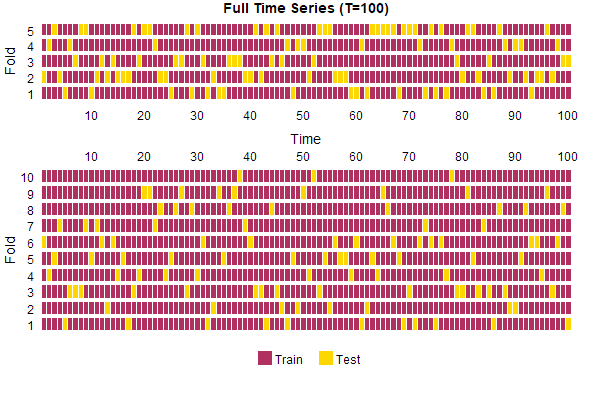
\includegraphics[scale=0.7]{kcvplots}
\end{figure}

Following similar notation from \cite{Hastie2009a}, $\kappa:\{m,m+1,\cdots,T\}\to\{1,\cdots,K\}$ is the indexing function mapping data to specific testing groups. An estimate of PE is obtained for each $\lambda \in \mathcal{L}$ and $\alpha \in \mathcal{A}$, and optimal tuning parameters are chosen based on minimization of this estimate. Specifically for the LASSO cases, $\widehat{PE}(\lambda)$ is expressed in Equation \ref{eq:lassocvpe}. We use $\hat{\bm{\beta}}_{\kappa(t)}(\lambda)$ to represent the estimated ARMA parameters from models fitted to data not in the $\kappa(t)$ group. The most exhaustive case is leave-one-out CV (LOOCV) where $K=(T-m+1)$ and  $\kappa(t)=t-m+1$. Obtaining $\widehat{PE}(\lambda)$ for LOOCV would be time consuming if not for the generalized CV (GCV) of \cite{Wahba1978}.

\begin{equation}
\label{eq:lassocvpe}
	\widehat{PE}(\lambda)=\frac{1}{T-m+1}\sum\limits_{t=m}^T \bigg(y_t-\bm{x}_t'\hat{\bm{\beta}}_{\kappa(t)}(\lambda)\bigg)^2
\end{equation}


\subsubsection{SELECTION BASED ON OUT-OF-SAMPLE EVALUATION}

Applied statisticians prefer CV-K or LOOCV when data is cross-sectional. This approach is not intuitive for time series data where prediction on a randomly selected subset of the full data does not seem like forecasting. For a particular $\tau\in (0,1)$, the out-of-sample (OOS) method estimates $\hat{\bm{\beta}}(\lambda)$ from the first $(1-\tau)\times 100\%$ of the data (TRAIN) and forecasts on the final $\tau\times 100\%$ (TEST). Equation 
\ref{eq:lassooos} equates to mean squared forecast error (MSFE) and is used to optimally select tuning parameters. 
\begin{equation}
\label{eq:lassooos}
	\widehat{PE}(\lambda)=\frac{1}{\tau T}\sum\limits_{t\in \textrm{TEST}} \bigg(y_t-\bm{x}_t'\hat{\bm{\beta}}(\lambda)\bigg)^2
\end{equation}

For subset ARMA selection, order parameters $p$ and $q$ are fixed and quantify the memory required to forecast.  In our naive description of OOS, we ignore the fact that some of our forecasts in the TEST period are obtained using data in the TRAIN period. Given $p$ and $q$, the final $d=\max\{p,q\}$ points in the TRAIN period are ignored in model fitting. Now, models are strictly evaluated on future data independent of the TRAIN period. In some literature, this is default OOS \citep{Bergmeir2018}; however, we abbreviate this modified version depOOS to highlight the additional considerations being made. Figure \ref{fig:oosplots} displays the difference data division between OOS and depOOS.

\begin{figure}[htbp!]
	\caption{Variations of Out-of-Sample Procedures for Model Selection}
	\label{fig:oosplots}
	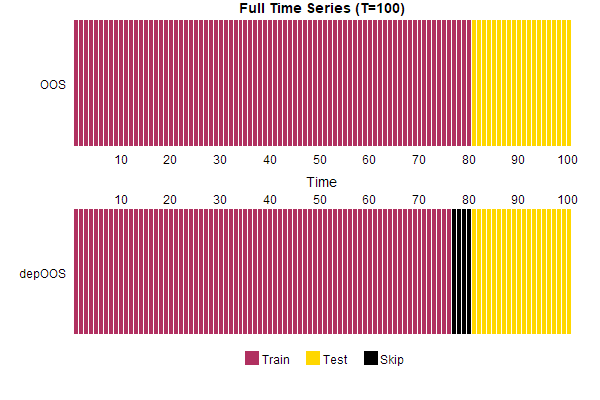
\includegraphics[scale=0.7]{oosplots}
\end{figure}


\subsubsection{SELECTION BASED ON BLOCKED CV}
Classic CV estimates the expected PE constructed from predictions on unfitted data. This may lead to a poor estimate for time series data where the popular "independent observation" assumption is violated \citep{Arlot2010}. \cite{Burman1994} modified LOOCV by ignoring the $d$ observations before and after each time point in fitting. Similarly, \cite{Bergmeir2018} describe and evaluate a non-dependent version CV-K. For $T-m+1=100$ and $d=4$, we show this modification in Figure \ref{fig:depkcvplots} which is based off the same random assignment in Figure \ref{fig:oosplots}. Controlling the number of points available for fitting models is difficult for this modified CV-K even for a low order $d$. This along with the poor empirical results in \cite{Bergmeir2018} removes this approach from consideration.

\begin{figure}[htbp!]
	\caption{Non-Dependent $K$-fold Cross-Validation for Model Selection for $K=5$ (top) and $K=10$ (bottom)}
	\label{fig:depkcvplots}
	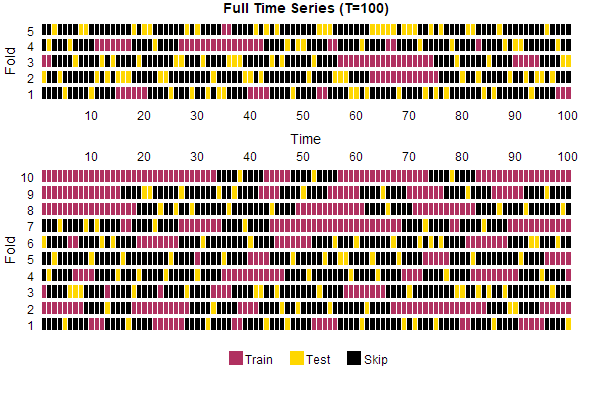
\includegraphics[scale=0.7]{depkcvplots}
\end{figure}

In this paper, we propose blocked variants of CV that retain the ordered structure and ensure reasonable sample sizes for model fitting. \cite{Racine2000} alters the CV method of \cite{Burman1994} to measure prediction error on blocks of data around each data point for each fold. \cite{Bergmeir2012} proposes K-fold blocked CV (BCV-K) where naturally ordered data is evenly split into $K$ sets.  For order $d$, the first and last $\lceil \frac{d}{2} \rceil$ data points are removed from each block to remove dependence, and ordinary CV is performed using the blocks. See Figure \ref{fig:bcvplots} for for BCV-5 and BCV-10 when $d=4$. 

\begin{figure}[htbp!]
	\caption{Non-Dependent $K$-Block Cross-Validation for Model Selection for $K=5$ (top) and $K=10$ (bottom)}
	\label{fig:bcvplots}
	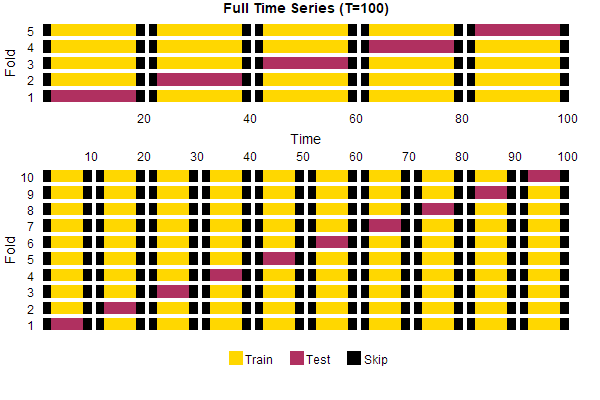
\includegraphics[scale=0.7]{bcvplots}
\end{figure}

Analogous to LOOCV, we extend BCV-K to leave-one-block-out CV (LOBOCV) design. This approach is similar to BCV-$K^*$ when $K^*=\lfloor \frac{T-m+1}{d} \rfloor$ since we divide time series sequentially into $K^*$ blocks. Block specific estimates $\widehat{PE}_K(\lambda)$ or $\widehat{PE}_K(\lambda,\alpha)$ are evaluated after models are fitted to data in non-adjacent blocks. In LASSO cases, overall BCV prediction error is based on expression in Equation \ref{eq:lobocv2}. Similar expressions are seen for BCV-5 and BCV-10 since all prediction periods are of the same length. This is a key difference to the initial proposed non-dependent CV-K.

\begin{equation}
\label{eq:lobocv2}
	\widehat{PE}(\lambda)=\frac{1}{K}\sum\limits_{k=1}^K \widehat{PE}_K(\lambda)
\end{equation}

\begin{figure}[htbp!]
	\caption{Leave-One-Block-Out Cross-Validation for Model Selection}
	\label{fig:lobocvplots}
	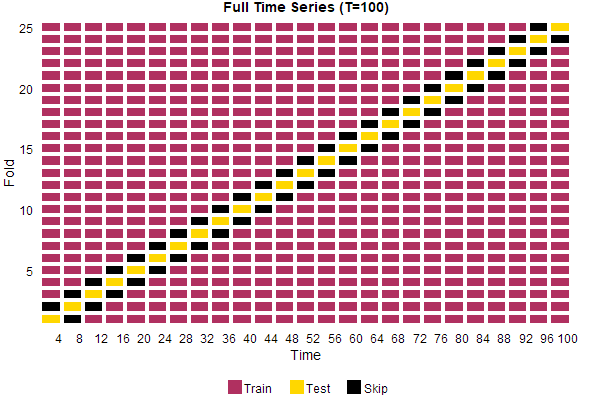
\includegraphics[scale=0.7]{lobocvplots}
\end{figure}

Literature evaluates these methods on the error between estimated $\widehat{PE}$ using CV and OOS and true $PE$ from data completely ignored \citep{Bergmeir2014,Bergmeir2018}. Typical experiments examine this error when the fitted models are known to be misspecified \citep{Burman1994,Racine2000,Bergmeir2018}. These discussions are not the focus on this paper. We only explore the performance of these methods in selection of $\lambda$ and $\alpha$ for ADLASSO and ADENET. 

\subsection{BAYESIAN PREDICTIVE POSTERIOR PROJECTION METHOD}
\subsubsection{TRADITIONAL BAYESIAN MODEL SELECTION}
Classic Bayesian model selection starts by reparamaterizing $\beta_i^*=\xi_i\beta_i$ where $\xi_i\in\{0,1\}$. For the new vector of parameters $\bm{\beta}^*=[\beta^*_1,\beta^*_2,\cdots,\beta^*_{p+q}]'$, the set of relevant parameters $\mathcal{V}=\{i:\beta^*_i\neq 0\}=\{i:\xi_i\neq 0\}$. Let $\mathcal{N}_p(\bm{\mu},\sigma^2\bm{\Sigma}_p)$ represent the $p$-dimensional multivariate normal distribution and $BERN(\pi)$ represent the Bernouilli distribition. If dimension $p$ is not given, assume $p=1$. The scenario $\bm{\Sigma}_p=\bm{I}_p$, where $\bm{I}_p$ is $p\times p$ identity matrix, implies that $\beta_j\perp\beta_k$ for all $j\neq k$. For the new linear model  $\bm{y}=\bm{X}\bm{\beta}^*$, \cite{Kuo1998} suggested the prior $p(\beta_i,\xi_i)=p(\beta_i)p(\xi_i)$ indicating $\beta_i \perp \xi_i$. Later authors suggested $p(\beta_i,\xi_i)=p(\beta_i|\xi_i)p(\xi_i)$ where $p(\beta_i|\xi_i)=(1-\xi_i)p(\beta_i|\xi_i=1)+\xi_i p(\beta_i|\xi_i=0) $ is a mixture prior \citep{Carlin1995}. The popular "spike and slab" prior is of this type where the slab $p(\beta_i|\xi_i=1)$ is uninformative and the spike $p(\beta_i|\xi_i=0)$ is concentrated around 0 \citep{Mitchell1988,George1993, Carlin1995}. Common to all methods, $\xi_i \sim BERN(\pi_{i,0})$ where $\pi_{i,0}$ is the prior probability that variable $\beta_i \neq 0$. All subset models are equally likely \textit{a priori} when $\pi_{i,0}=0.5$. Sampling from $p(\bm{\beta},\bm{\xi},\sigma^2|\bm{y},\bm{X})$ requires a combination of approaches \citep{Dellaportas2002}, and the posterior mode of $\bm{\xi}$ indicates the best model. Posterior model probabilities and Bayes factors are used to discriminate between possible sub models. Implementation of Bayesian model averaging is within this umbrella \citep{Raftery1997,Hoeting1998,Hoeting1999}.

\subsubsection{BAYESIAN REGULARIZATION}
Posterior samplers based on 2-component mixture priors are often slow in exploring high-dimensional spaces. Priors developed from continuous mixing densities achieve similar results without requiring tuning. For example, \cite{Andrews1974} presented a hierarchy for the $Laplace$ (i.e. $Double-Exponential$) distribution from scale-mixture of $Normals$ using $Exponential$ mixing density. The Bayesian LASSO \citep{Park2008,Hans2009} uses this hierarchy for $p(\bm{\beta}|\sigma^2)$ understanding the link between $\ell_1$-regularization and posterior modes from $Laplace$ priors \citep{Tibshirani1996}. See \cite{OHara2009} for a historical look and comparison of adaptive Laplacian priors to discontinuous mixture priors.

Since the introduction of Bayesian LASSO, research in Bayesian regularization methods has exploded over the last ten years. Bayesian methods analogous to adaptive lasso \citep{Leng2014}, elastic net \citep{Li2010a}, and adaptive elastic net \citep{Stankiewicz2015} have been introduced and applied. The prior hierarchies of the aforementioned methods are in a class of "global-local" shrinkage priors \citep{Polson2010}. The recently popular Bayesian horseshoe (BHS) prior falls in this class where $half-Cauchy$ priors are used to enforce global sparsity while preventing overshrinking of relevant parameters \citep{Carvalho2009,Carvalho2010}. The BHS enjoys the important oracle properties established for ADLASSO and ADENET \citep{Datta2015}. \cite{Bhadra2016} introduced horseshoe+ ($\textrm{BHS}^+$) which includes an additional layer of local shrinkage improving estimation when $\bm{\beta}$ is "ultra-sparse". In subset ARMA selection, we safely choose $p$ and $q$ large enough to ensure any long lag seasonal effects may be discovered. Overestimation of $p$ and $q$ may introduce many non-seasonal ARMA terms that are equal to 0.  For these reasons, we utilize BHS and $\textrm{BHS}^+$ type priors for $\beta_i$. 

The hierarchical representations of BHS and $\textrm{BHS}^+$ displayed in Equations \ref{eq:makschmidths} \& \ref{eq:makschmidthsp} allow posterior sampling via Gibbs \citep{Makalic2016b}. These hierarchies developed from understanding that $\tau^2|\xi \sim \mathcal{IG}(1/2,1/\xi)$ and $\xi\sim\mathcal{IG}(1/2,1/a)$ imply $\tau\sim\mathcal{C}^+(0,a)$ \citep{Wand2011}. Expressions $\mathcal{IG}(a,b)$ and $\mathcal{C}^+(0,a)$ represent $inverse-gamma$ and $half-Cauchy$ distributions, respectively. The latent parameter $\tau$ controls overall regularization. Global shrinkage parameter $\tau$ can be fixed \citep{vanderPas2014}, updated via empirical Bayes \citep{Johnstone2004}, or given a hyperprior\citep{Carvalho2009,Carvalho2010}. Prior beliefs on the degree of sparsity in $\bm{\beta}$  should drive the handling of $\tau$ improving regularization \citep{vanderPas2014,Piironen2016}. The additional latent parameters $\lambda_i$ fine tune the regularization induced by $\tau$ for individual $\beta_i$. Heavy-tails of $\mathcal{C}^+(0,1)$ prevent relevant ARMA parameters from being overshrunk to 0.
\begin{equation}
\label{eq:makschmidths}
\begin{split}
\bm{y}|\bm{X},\bm{\beta},\sigma^2 & \sim \mathcal{N}_{p+q}(\bm{X}\bm{\beta},\sigma^2\bm{I}_{p+q}) \\
\beta_i|\lambda^2_i,\tau^2,\sigma^2 & \sim \mathcal{N}(0,\lambda^2_i\tau^2\sigma^2) \\
\sigma^2 & \sim \sigma^{-2}\textrm{d}\sigma^2 \\
\lambda^2_i|\nu_i & \sim \mathcal{IG}(1/2,1/\nu_i)\\
\tau^2|\xi & \sim \mathcal{IG}(1/2,1/\xi)\\
\nu_1,\cdots, \nu_{p+q}& \sim \mathcal{IG}(1/2,1) \\
\xi & \sim \mathcal{IG}(1/2,1) \\
\end{split}
\end{equation}
\begin{equation}
\label{eq:makschmidthsp}
\begin{split}
\bm{y}|\bm{X},\bm{\beta},\sigma^2 & \sim \mathcal{N}_{p+q}(\bm{X}\bm{\beta},\sigma^2\bm{I}_{p+q}) \\
\beta_i|\lambda^2_{1,i},\lambda^2_{2,i},\tau^2,\sigma^2 & \sim \mathcal{N}(0,\lambda^2_{1,i}\lambda^2_{2,i}\tau^2\sigma^2) \\
\sigma^2 & \sim \sigma^{-2}\textrm{d}\sigma^2 \\
\lambda^2_{1,i}|\nu_{1,i} & \sim \mathcal{IG}(1/2,1/\nu_{1,i})\\
\lambda^2_{2,i}|\nu_{2,i} & \sim \mathcal{IG}(1/2,1/\nu_{2,i})\\
\tau^2|\xi & \sim \mathcal{IG}(1/2,1/\xi)\\
\nu_{1,i},\cdots, \nu_{1,p+q} & \sim \mathcal{IG}(1/2,1) \\
\nu_{2,i},\cdots, \nu_{2,p+q} & \sim \mathcal{IG}(1/2,1) \\
\xi & \sim \mathcal{IG}(1/2,1) \\
\end{split}
\end{equation}

\subsubsection{PREDICTIVE POSTERIOR PROJECTION METHOD}

Define $\mathcal{V}_F=\{1,2,\cdots,p+q\}$. For the fully saturated ARMA$(p,q)$ model, let $\hat{\bm{\beta}}_{HS}(\mathcal{V}_F)$ and $\hat{\bm{\beta}}_{HS^{+}}(\mathcal{V}_F)$ correspond to the posterior means of $\bm{\beta}$ under BHS and $\textrm{BHS}^+$, respectively. Both $\hat{\bm{\beta}}_{HS}(\mathcal{V}_F)$ and $\hat{\bm{\beta}}_{HS^{+}}(\mathcal{V}_F)$ are quality initial estimates of $\bm{\beta}$ but not sparse since $\hat{\beta}_i \neq 0$ for all $i$. Obtaining these estimates is analogous to the first stages of ADLASSO and ADENET. Any $\mathcal{V}_\perp \subset \mathcal{V}_F$ characterizes a particular subset ARMA$(p,q)$ model via indicating the parameters of $\bm{\beta}$ included.  Although the best model $\mathcal{V}^* \subset \mathcal{V}_F$ may differ under BHS and $\textrm{BHS}^+$, the corresponding final subset ARMA$(p,q)$ models are defined $\hat{\bm{\beta}}_{HS}=\hat{\bm{\beta}}_{HS}(\mathcal{V}^*)$ and $\hat{\bm{\beta}}_{HS^{+}}=\hat{\bm{\beta}}_{HS^{+}}(\mathcal{V}^*)$. In this section, we present a Bayesian inspired algorithm to select $\mathcal{V}^*$ after an initial BHS or $\textrm{BHS}^+$ estimation. For simplicity, we generalize an outline of this approach for both BHS and $\textrm{BHS}^+$.

After Bayesian estimation, the full model $\mathcal{V}_F$ represents a viable reference model. The sets $\{\bm{\beta}^{(s)}(\mathcal{V}_F)\}_{s=1}^S$ and $\{\sigma^{(s)}(\mathcal{V}_F)\}_{s=1}^S$ are the $S$ posterior samples under the reference model. Given a proposed nested model $\mathcal{V}_\perp \subset \mathcal{V}_F$, \cite{Goutis1998} suggested the Kullback-Leibler (K-L) distance \citep{Kullback1951} to evaluate discrepancy between $\mathcal{V}_F$ and $\mathcal{V}_\perp$. Classic model selection via AIC is based on K-L information and derivable from a Bayesian perspective \citep{Akaike1974,Akaike1985,burnham2003,Burnham2004}. For a future value $\tilde{y}=y_{T+1}$, we measure the loss of explanatory power of using of $\mathcal{V}_\perp$ instead of $\mathcal{V}_F$  by assessing the K-L distance between the posterior predictive distributions listed in Equation \ref{eq:projpreddist}. If the discrepancy between $p(\tilde{y}|\bm{y},\bm{X},V_F)$ and $p(\tilde{y}|\bm{y},\bm{X},V_\perp)$ is small, the more parsimonious $\mathcal{V}_\perp$ is favored.  The foundation of this concept is provided in \cite{Dupuis2003,Nott2010,vehtari2012,Piironen2015b,Piironen2017}.
\begin{equation}
\label{eq:projpreddist}
\begin{split}
p(\tilde{y}|\bm{y},\bm{X},V_F)&=\int\int p(\tilde{y}|\bm{y},\bm{X},\bm{\beta}_F,\sigma_\perp,V_F)p(\bm{\beta}_F,\sigma_F|\bm{y},\bm{X},V_F) \textrm{ d}\bm{\beta}_F \textrm{ d}\sigma_F\\
p(\tilde{y}|\bm{y},\bm{X},V_\perp)&=\int\int p(\tilde{y}|\bm{y},\bm{X},\bm{\beta}_\perp,\sigma_\perp,V_\perp)p(\bm{\beta}_\perp,\sigma_\perp|\bm{y},\bm{X},V_\perp) \textrm{ d}\bm{\beta}_\perp \textrm{ d}\sigma_\perp\\
\end{split}
\end{equation}


For Gaussian linear models, $S$ posterior samples $\{\bm{\beta}^{(s)}(\mathcal{V}_\perp)\}_{s=1}^S$ and $\{\sigma^{(s)}(\mathcal{V}_\perp)\}_{s=1}^S$ for a nested submodel $\mathcal{V}_\perp$ are quickly obtained via Equation \ref{eq:projform}  \citep{Piironen2015b}. The matrix $\bm{X}_\perp$ contains the columns of the reference model matrix $\bm{X}$ corresponding to $\mathcal{V}_\perp$. Essentially, we are obtaining $S$ samples from the posterior distribution of a submodel through projecting the fitted values from the full model  onto a smaller parameter space.
\begin{equation}
\label{eq:projform}
\begin{split}
	\bm{\beta}^{(s)}(\mathcal{V}_\perp) &= (\bm{X}'_\perp\bm{X}_\perp)^{-1}\bm{X}'_\perp\bm{X}\bm{\beta}^{(s)}(\mathcal{V}_F) \\
	\sigma^{(s)}(\mathcal{V}_\perp) &=\sqrt{[\sigma^{(s)}(\mathcal{V}_\perp)]^2+\frac{||\bm{X}\bm{\beta}^{(s)}(\mathcal{V}_F)-\bm{X}_\perp \bm{\beta}^{(s)}(\mathcal{V}_\perp)||^2}{T-m+1}}
\end{split}
\end{equation}

The overall discrepancy between the full ARMA$(p,q)$ model and a subset ARMA$(p,q)$ model is measured in Equation \ref{eq:deltaform}. Here we are estimating the expected KL divergence between the predictive distribution of the $\mathcal{V}_F$ and $\mathcal{V}_\perp$.
\begin{equation}
\label{eq:deltaform}
	D(\mathcal{V}_F||\mathcal{V}_\perp)=\frac{1}{S}\sum\limits_{s=1}^S \log\bigg(\frac{\sigma^{(s)}(\mathcal{V}_\perp)}{\sigma^{(s)}(\mathcal{V}_F)}\bigg)
\end{equation}

Measuring the discrepancy in Equation \ref{eq:deltaform} for all $2^{p+q}-1$ subset ARMA models is impractical; therefore, we favor the forward stepwise algorithm of \cite{Peltola2014}. If $\mathcal{V}_0$ represents the intercept-only model (empty model in our case), we know $D(\mathcal{V}_F||\mathcal{V}_0)$ is the maximum discrepancy for all possible $\mathcal{V}_\perp$ \citep{Dupuis2003}. Next, we select the best subset ARMA model with one additional parameter by Equation \ref{eq:step1}.
\begin{equation}
\label{eq:step1}
\mathcal{V}_1=\underset{\{\mathcal{V}_0\subset\mathcal{V}_\perp\subset \mathcal{V}_F :|\mathcal{V}_\perp|=1\}}{\textrm{argmin}}D(\mathcal{V}_F||\mathcal{V}_\perp)
\end{equation}
Moving forward to models with two additional parameters, we identify the best subset ARMA model with 2 ARMA parameters by Equation \ref{eq:step2}.
\begin{equation}
\label{eq:step2}
\mathcal{V}_2=\underset{\{\mathcal{V}_1\subset\mathcal{V}_\perp\subset \mathcal{V}_F :|\mathcal{V}_\perp|=2\}}{\textrm{argmin}}D(\mathcal{V}_F||\mathcal{V}_\perp)
\end{equation}
In general, the best subset ARMA model with $m$ coefficients, identified $\mathcal{V}_m$, where $\mathcal{V}_{m-1}\subset\mathcal{V}_m \subset \mathcal{V}_{m+1}$, based on Equation \ref{eq:step3}. \cite{Piironen2015} present a helpful tutorial of this approach with {\bf R} code and application.
\begin{equation}
\label{eq:step3}
\mathcal{V}_m=\underset{\{\mathcal{V}_{m-1}\subset\mathcal{V}_\perp\subset \mathcal{V}_F :|\mathcal{V}_\perp|=i\}}{\textrm{argmin}}D(\mathcal{V}_F||\mathcal{V}_\perp)
\end{equation}


The forward stepwise algorithm leads to the following sequence of $p+q$ nested models: $\mathcal{V}_1 \subset \cdots \subset \mathcal{V}_F$. Because of the additive property of $D(\cdot||\cdot)$, \cite{Dupuis2003} recommend selecting $\mathcal{V}^* \in \{\mathcal{V}_1,\cdots,\mathcal{V}_F\}$ based on the relative explanatory power ($e$) defined in Equation \ref{eq:RelEform}. 
\begin{equation}
\label{eq:RelEform}
\begin{split}
e(\mathcal{V}_{m})&=1-\frac{D(\mathcal{V}||\mathcal{V}_m)}{D(\mathcal{V}||\mathcal{V}_0)}\\
\end{split}
\end{equation}
This additive property ensures $0=e(\mathcal{V}_{0}) < e(\mathcal{V}_{m})< e(\mathcal{V}_{F})=1$ for any $m\in\{1,\cdots,p+q-1\}$. For an acceptable explanatory power $e^*$, we select $\mathcal{V}^*=\mathcal{V}_{m^*}$ based on $m^*$ defined in Equation \ref{eq:bestRelEform}. \cite{Piironen2015} suggest $e^*\geq 0.90$.  In our empirical studies, we examine the model selection sensitivity for $e^*\in\{0.9,0.95,0.98\}$.
\begin{equation}
\label{eq:bestRelEform}
m^*=\min \{m: e(\mathcal{V}_{m})>e^*\}
\end{equation}

In an application to biomarker identification for cardiovascular event risk, \cite{Peltola2014} based model selection from estimating predictive performance via 10-fold CV. Combining Bayesian techniques with multi-fold CV is time consuming, and the validity of general CV in time series analysis is questionable. Using the same OOS and depOOS schemes illustrated in Figure \ref{fig:oosplots}, we intentionally withhold a final portion of the data for forecast evaluation. We estimate PE for each nested model using MSFE according to Equation \ref{eq:hsoos}. Although we lose  $\tau\times 100\%$ of the data in estimation, the final model $\mathcal{V}^*$ must demonstrate superior OOS forecasting performance to the other $p+q$ candidates.
\begin{equation}
\label{eq:hsoos}
	\widehat{PE}(\mathcal{V})=\frac{1}{\tau T}\sum\limits_{t\in \textrm{TEST}} \bigg(y_t-\bm{x}_t'\hat{\bm{\beta}}_{HS}(\mathcal{V})\bigg)^2
\end{equation}












\subsection{SUMMARY}

In this section, we included OOS and CV techniques for choosing tuning parameters. Table \ref{tab:aicbic} lists the gamut of options discussed and tested in Monte Carlo simulations. For future reference, we abbreviate the 2-stage ADLASSO and ADENET variants $\textrm{AL}_m$ and $\textrm{AE}_m$ where $m \in \{1,2,\cdots,11\}$ identifies the method. 

\begin{table}[!h]
  \footnotesize
  \centering
  \caption{Summary of ADLASSO and ADENET Variants}
    \begin{tabular}{c|cc}
    \toprule
    Method ($m$) & Initial Weights (Stage 1) & Final Model (Stage 2)  \\
    \midrule
    1 & AIC & AIC\\
    2 & AIC & BIC \\
    3 & BIC & BIC \\
    \midrule
    4 & \multicolumn{2}{c}{OOS} \\
    5 & \multicolumn{2}{c}{depOOS} \\
    \midrule
    6 & \multicolumn{2}{c}{CV-5} \\
    7 & \multicolumn{2}{c}{CV-10} \\
    8 & \multicolumn{2}{c}{LOOCV} \\
    \midrule
    9 & \multicolumn{2}{c}{BCV-5} \\
    10 & \multicolumn{2}{c}{BCV-10} \\
    11 & \multicolumn{2}{c}{LOBOCV} \\
    \bottomrule
    \end{tabular}%
  \label{tab:aicbic}%
\end{table}%

Additional methods considered are from a Bayesian perspective. Initial posterior sampling is based off either BHS or $\textrm{BHS}^+$ priors. Table \ref{tab:bhstypes} lists different options for final model selection in the predictive posterior projection method. For future reference, we abbreviate Bayesian options $\textrm{BHS}_m$ and $\textrm{BHS}^+_m$ where $m \in \{1,2,\cdots,5\}$. 

\begin{table}[!h]
  \footnotesize
  \centering
  \caption{Summary of BHS and $\textrm{BHS}^+$ Variants }
    \begin{tabular}{c|cc}
    \toprule
    Method ($m$) & Final Model Selection  \\
    \midrule
    1 & $e(\cdot)>0.90$ \\
    2 & $e(\cdot)>0.95$ \\
    3 & $e(\cdot)>0.98$\\
    \midrule
    4 & OOS\\
    5 & depOOS\\
    \bottomrule
    \end{tabular}%
  \label{tab:bhstypes}%
\end{table}%








\section{MONTE CARLO SIMULATIONS}
\label{sec:mc}
Multiple Monte Carlo studies are performed to evaluate and compare ADLASSO, ADENET, and BPP on subset ARMA selection. Consider the three time series $\{y_{1,t}\}$, $\{y_{2,t}\}$, and $\{y_{3,t}\}$ generated by the Gaussian ARMA processes expressed in Equations \ref{eq:simarma1}, \ref{eq:simarma2}, and \ref{eq:simarma3} and abbreviated Models I, II, and III, respectively.
\begin{equation}
	\label{eq:simarma1}
	y_{1,t}=0.8y_{1,t-1}+0.7y_{1,t-6}-0.56y_{1,t-7}+\epsilon_{1,t}
\end{equation}
\begin{equation}
	\begin{split}
	\label{eq:simarma2}
	y_{2,t}&=0.8y_{2,t-1}+0.7y_{2,t-6}-0.56y_{2,t-7}\\
	&+0.8\epsilon_{2,t-1}+0.7\epsilon_{2,t-6}+0.56\epsilon_{2,t-7}+\epsilon_{2,t}
	\end{split}
\end{equation}
\begin{equation}
	\label{eq:simarma3}
	y_{3,t}=0.8\epsilon_{3,t-1}+0.7\epsilon_{3,t-6}+0.56\epsilon_{3,t-7}+\epsilon_{3,t}
\end{equation}
The errors $\{\epsilon_{1,t}\}$, $\{\epsilon_{2,t}\}$, and $\{\epsilon_{3,t}\}$ are i.i.d. Gaussian processes with $0$ mean and variance $\sigma^2$. Models I, II, and III are algebraically equivalent to the first three SARMA$(p,q)\times(P,Q)_6$ models found in \cite{Chen2011}, and similarly, we generate samples from these models of length $T\in \{120, 240, 360\}$ in our Monte Carlo experiments. Furthermore, we consider different choices for $\sigma\in\{0.5,1,1.5\}$ to explore sensitivity to noise. 

The proxy innovations $\{\hat{\epsilon}_{k,t}\}$ are obtained from long AR$(p^\prime)$ models where $p^\prime=10\log_{10}(T)$. Contrary to \cite{Chen2011}, better performance was observed when $p^\prime$ is fixed versus model selection via AIC. Estimation of $\bm{\phi}^\prime$ is obtained from Yule-Walker equations for ADLASSO and ADENET, and from Bayesian linear regression for BPP.

Results from both frequentist approaches heavily depend on the estimated weights $\hat{\bm{w}}=(|\tilde{\bm{\beta}}|+1/T)^{-\eta}$. Suggested by \cite{Zou2006} and used in \cite{Chen2011}, we only consider $\eta=2$. Specifically for ADLASSO, best empirical performance across all experiments occurred when $\tilde{\bm{\beta}}=\tilde{\bm{\beta}}_{LASSO}$ \citep{Chen2011}; therefore, we do not consider LS and RIDGE based weights in our study. In regards to ADENET, we experiment with both ENET and LASSO estimated $\tilde{\bm{\beta}}$.










\section{APPLICATION}
\label{sec:co2app}
Carbon dioxide $\textrm{CO}_2$ levels are constantly measured at strategically placed atmospheric monitoring observatories around the world to track climate change. The {\bf datasets} package in {\bf R} \citep{RCORETEAM} contains a monthly time series of  $\textrm{CO}_2$ levels for January 1959 to December 1997 measured in Mauna Loa, Hawaii, United States. The {\bf TSA} package in {\bf R} \citep{RTSA} contains a similar but shorter series  measured  in Alert, Nunavut, Canada, from January 1994 to December 2004. Let $\{x_{1,t}:t=1,2,\cdots,468\}$ represent the Mauna Loa data, and $\{x_{2,t}:t=1,2,\cdots,132\}$ represent the Alert data. Both $\{x_{1,t}\}$ and $\{x_{2,t}\}$ are nonstationary in mean and cyclical with seasonal periodicity $S=12$. The latter series $\{x_{2,t}\}$ serves as a primary textbook example  to demonstrate the selection, fitting, and forecasting of seasonal models \citep{Cryer2008}. Following the examples provided in \cite{Cryer2008,Chen2011}, subset SARMA$(p,q)\times(P,Q)_{12}$ models utilized at both locations are applied after seasonal and regular differencing . 

Define $y_{k,t}=\Delta_1\Delta_{12}x_{k,t}$ for $k\in\{1,2\}$  where $\Delta_s$ is the difference operator such that $\Delta_s y_t=y_t-y_{t-s}$.  Using all variations of adaptive lasso, adaptive elastic net, and projection model selection, we fit subset ARMA($14,14$) models to $\{y_{1,t}:t=1,2,\cdots,372\}$ corresponding to data prior to 1990 and $\{y_{2,t}:t=1,2,\cdots,108\}$ corresponding to data prior to 2003. The remaining portions $\{y_{1,t}:t=373,374,\cdots,468\}$ and $\{y_{2,t}:t=109,110,\cdots,132\}$ are intentionally preserved for forecasting comparison. Figures \ref{fig:co2plots} and \ref{fig:co2plots2} illustrate the division of the data into fitting and forecasting periods, as well as, the progression of seasonal and regular differencing for Mauna Loa and Alert, respectively.

\begin{figure}[htbp!]
	\centering
	\caption{Plots of $x_{1,t}$ (Top),$\Delta_{12}x_{1,t}$ (Middle), and $\Delta_1\Delta_{12}x_{1,t}$ (Bottom) Partitioned Into Fitting (solid) and Forecasting (dotted) Periods}
	\label{fig:co2plots}
	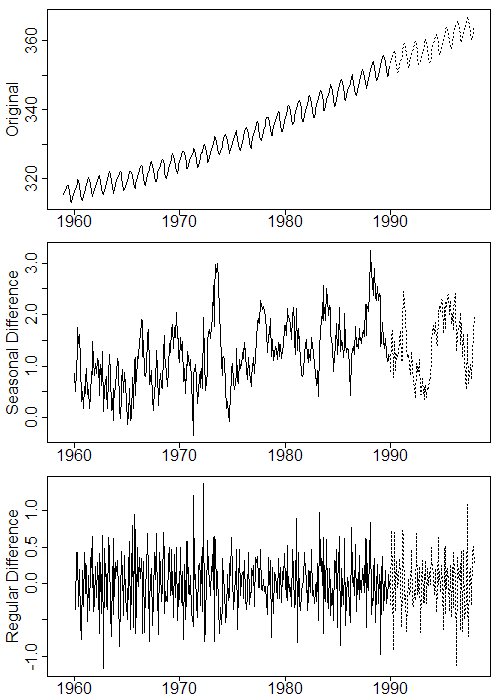
\includegraphics[scale=0.8]{co2plots}
\end{figure}

\begin{figure}[htbp!]
	\centering
	\caption{Plots of $x_{2,t}$ (Top),$\Delta_{12}x_{2,t}$ (Middle), and $\Delta_1\Delta_{12}x_{2,t}$ (Bottom) Partitioned Into Fitting (solid) and Forecasting (dotted) Periods}
	\label{fig:co2plots2}
	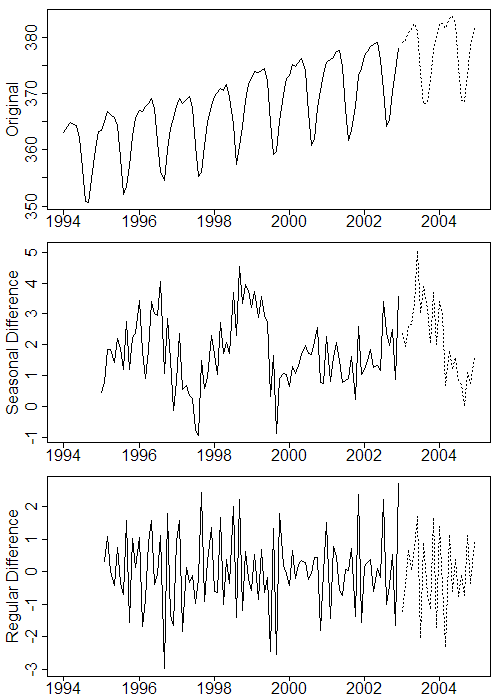
\includegraphics[scale=0.8]{co2plots2}
\end{figure}


The DGPs of $\{y_{1,t}\}$ and $\{y_{2,t}\}$ are hidden to the observer; therefore, evaluating the ability of a subset selection method to uncover the truth is an impossible task. The exploration into various cross-validation methods was motivated by the terminal desire to produce forecasts. Using the final subset ARMA($14,14$) models selected from the full library of methods presented in this paper, we obtain rolling $1$-step ahead predictions $\hat{y}_{k,t}$ over the full forecasting period of length $n_k$ where $k\in\{1,2\}$. As previously determined, $n_1=96$ and $n_2=24$.  Methods are evaluated based on root mean squared error (RMSE), mean absolute percentage error (MAPE), mean bias (MB), and mean directional bias (MDB). The formulas for these metrics are expressed in Equation \ref{eq:fmetrics}. In the expression for MDB, $\textrm{sgn}(x_t)=1$ if $x_t>0$ and $\textrm{sgn}(x_t)=-1$ if $x_t<0$.

\begin{equation}
\label{eq:fmetrics}
\begin{split}
	RMSE_k&=\frac{1}{n_k} \sum\limits_{j=1}^{n_k} (y_k-\hat{y}_k)^2 \\
	MAPE_k&=\frac{100}{n_k} \sum\limits_{j=1}^{n_k} \bigg|\frac{y_{k,j}-\hat{y}_{k,j}}{y_{k,j}}\bigg| \\
	MB_k&=\frac{1}{n_k} \sum\limits_{j=1}^{n_k} (y_{k,j}-\hat{y}_{k,j}) \\
	MDB_k&=\frac{1}{n_k} \sum\limits_{j=1}^{n_k} \textrm{sgn}(y_{k,j}-\hat{y}_{k,j})\\
\end{split}
\end{equation}







\section{CONCLUSION}
